% Lecture date: 04/15/2019, part one
% Authors: Yunhao Li, Geyi Zhang, He Li (editor)
% Time interval: 00:21:00 - 01:15:00
\chapter{Unsupervised Learning}

\section{Introduction}

\subsection{Machine Learning and the Cake Analogy}

Machine learning techniques such as supervised learning (which only predicts human-provided labels), and reinforcement learning (which only predicts a value function), are too narrow to create human-level intelligent machines. Unsupervised learning (or self-supervised learning to be exact), however, with its millions of bits of information per sample, can be used to train highly complex machines without human supervision.

Like supervised learning, self-supervised learning learns a function from pairs of inputs and outputs. However, instead of having annotators manually label the data, self-supervised learning automatically generates labels by extracting weak annotation information from the input data and predicting the rest. In this way the model can independently learn semantic feature representations of data, which can be further used in other tasks.

There are some examples where supervised learning is not suitable and we can use unsupervised learning techniques:
\begin{itemize}
    \item \textbf{Machine translation for any given language pair}: There are about 5k-7k languages, and we cannot do a supervised problem of learning $n^2$ language-to-language pair translators. A unsupervised learning way to do this is using a encoder-decoder structure we encode any language into a intermediate representation space ($n$ encoder) and decode from this internal representation to the chosen language ($n$ decoder).

    \item \textbf{Learning with very small amount of data}: There is a lot of situation that we don't have a lot of labeled data. People want to detect rare occurrences of things. Train a system to detect rare diseases in medical images or train the automatic driving systems where you cannot to exhaust every cases.

    \item \textbf{Combining deep learning with reasoning}: In some case we need to train systems to reason, not just perceive. Human have a pretty good model that predicts what may happen. So we can know the result without trying it. This model is acquired by observing which is a form of unsupervised learning.
\end{itemize}

Today’s AI technologies can easily classify images and recognize voices, but cannot perform tasks such as reasoning the relationship between different objects or predicting humans’ movements. That is where unsupervised learning can fill the blanks. The reason we need unsupervised learning is the fact that the number of the amount of the data we ask machine to predict is sort of different. These different paradigms of learning are very different.

\begin{itemize}
    \item In the reinforcement learning, you ask machine to predict a reward(cost) of a particular sequence of action. The system just gets a reward instead of much information in the end. It is a very sparse feedback, which means the number of trials needed is very large because in every trial you only give it a little information.

    \item In supervised learning, you give $10-10,000$ bits per sample. When doing ImageNet classification, for example, there is $1,000$ categories. The information is $10$ bits.

    \item In unsupervised learning, much more information has be used.
\end{itemize}

There is a analogy of machine learning and the cake: almost everything we learn we learned in unsupervised learning. We learn a little bit through supervised learning, and we learn a tiny bit through reinforcement learning.

\begin{figure}[ht]
\centering
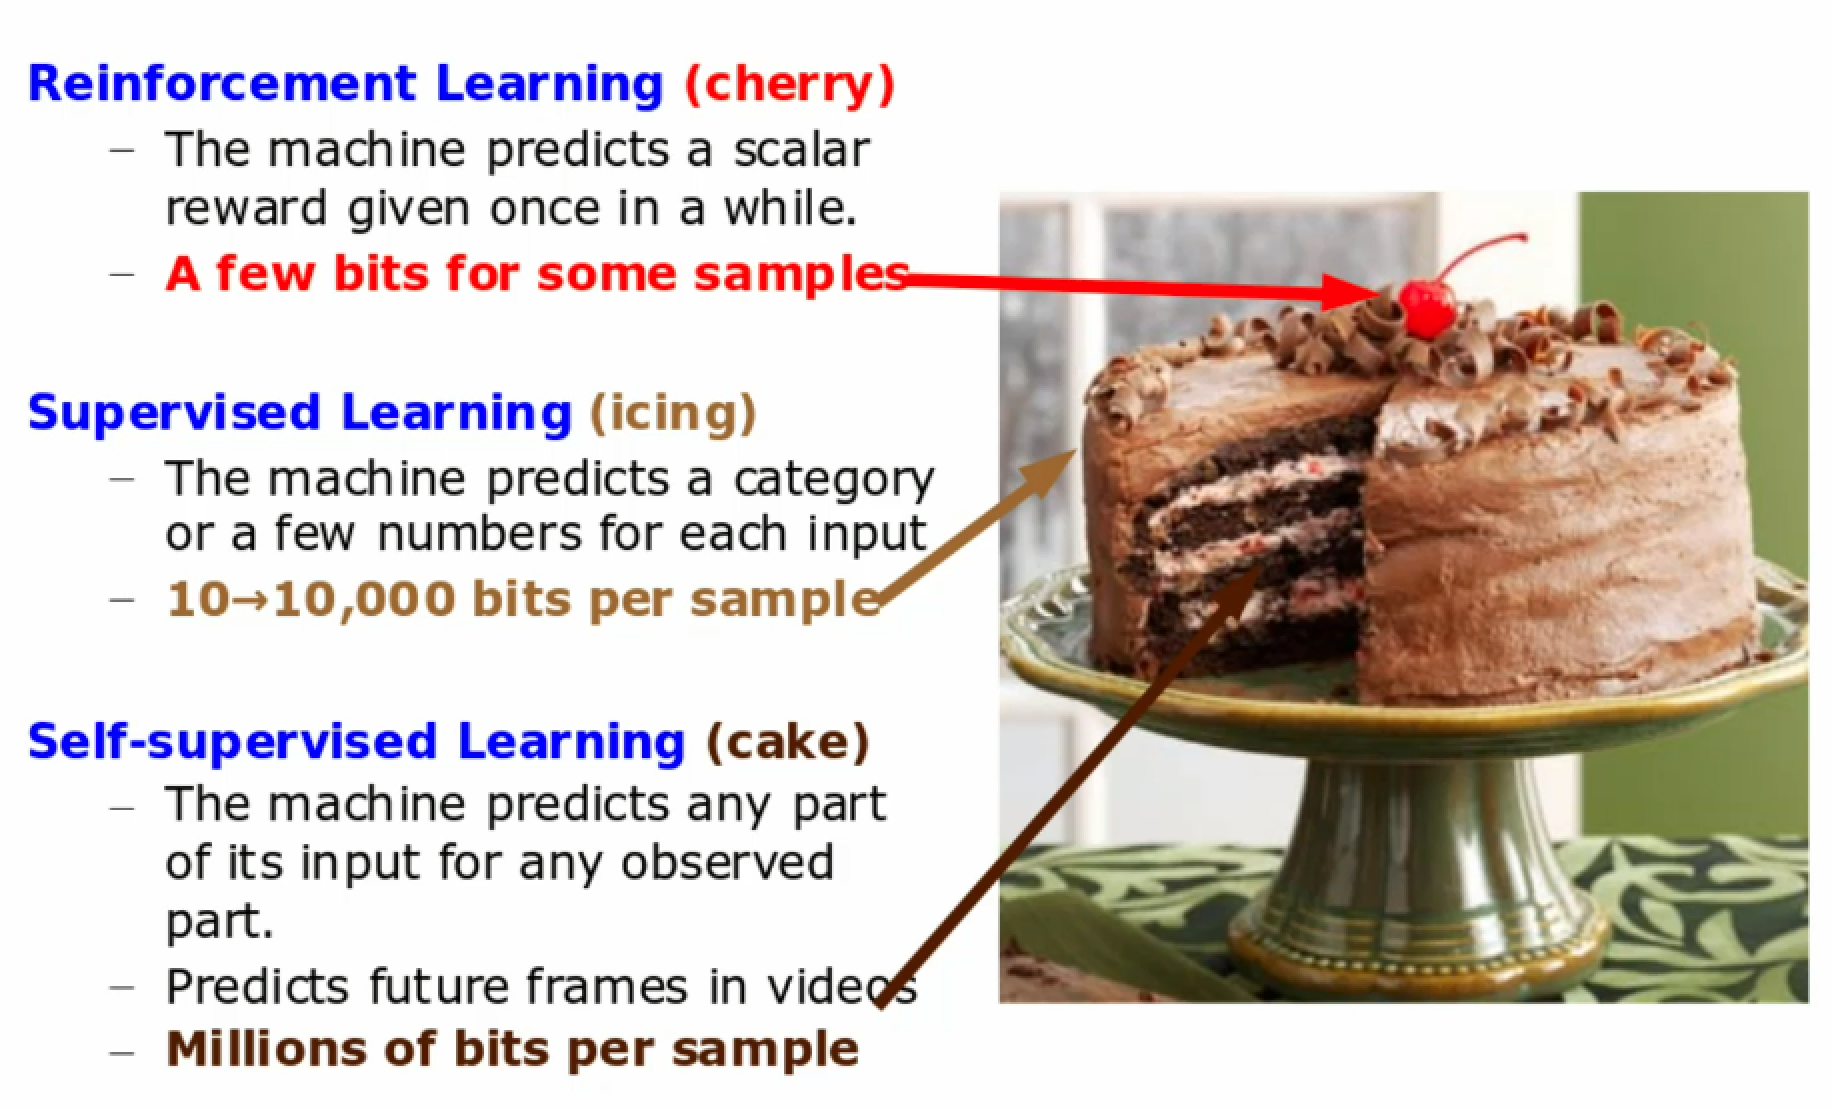
\includegraphics[height=7cm]{lectures/10-a/cake.png}
\caption{Cake Analogy}
\label{fig:label}
\end{figure}

\subsection{How do we do unsupervised learning?}

Prediction is kind of a reconstruction. For example, you can train a system to predict the end of a video from the beginning. But you can also do it in the other direction(given the end, predict what happened before). Completing the missing information, filling the blanks, that's the purpose of unsupervised learning.

So there is a problem: if I ask you to predict the future of a video with given video clips, many plausible things can happen. There is no single correct answer for this. The energy based learning will be useful. We need to construct a predictor that can predict multiple things, not just one single future prediction. The world is not entirely predictable. There is a lot of uncertainty. The question is, how do construct machine to predict things. The immediate answer is we can predict a distribution instead of predicting a single point.(e.g. Put a pen on table and let it go. The pen falls in a different direction every time. The directions is in a distribution) If you want to predict a frame of video, there is a distribution of images. You will have to parameterize the distribution of images. The basic possible to parameterize the distribution. We don't have density models or condition models of natural images. The main issue is that we don't know how to represent normalized distributions. Giving a quality of goodness or badness to a particular image is maybe possible, but training this into a distribution is very hard. That is one reason for introducing energy based models.

\section{Energy-based Unsupervised Learning}

\subsection{Introduction}

The way to make multiple predictions, or to build a model makes multiple predictions is through the latent variable. Imagine that for a predictor we are going to train, the $x$ are the frames of the video tape, $y$ is the feature of that particular video tape, and we will have an extra input $z$ to the function. What we would like to have is training the system in such a way that, when the latent variable varies over a particular set, the output varies over the set of all plausible predictions. For a particular $z$, the predicted next frame $y^\prime$ and the actual $y$ observed, by tweaking the latent variable, the model is to predict the actually observed $y$.

The idea of latent variable model is that, we have a latent variable of which value is not known, but through optimization, you are able to find the value of it that makes the best prediction.

What to do here is to measure the distance, try to figure out what is the value $z$ within the set, that would minimize the distance between the prediction $y^\prime$ and the $y$ observed. It may not actually be equal, so you will train the network to make these two as closet as possible, for the particular $z$.

\subsection{Shape the Energy Function}

The energy-based unsupervised learning is identical to energy-based models, except here are $Y_1$ and $Y_2$ instead of $X$ and $Y$. We train the network to figure out the structure of $Y$, where the energy function will takes low values of the data points nearby and higher values that aside. Capturing those dependencies through the energy function allows you to predict any subset of variables from any other subset of variables.

Making energy low on the training samples is easy, which can be achieved just by showing the training data and tweaking the parameters to make energy low on them. The most tricky part is how to ensure the energy is higher outside the training data. There are several ways to do that as shown below.

\begin{enumerate}
    \item \textbf{Constant and Constraint}: The volume of the space that your energy function can give low values to is limited or constant. For example, normalized probability model satisfy this condition, because if at one point the probability goes up, there would be another point that goes down to maintain the normalized distribution. Since the whole volume of probability is constant which equal to $1$, the volume of low energy stuff is constant as well.
    \begin{enumerate}
        \item \textbf{Gaussian Mixture Model}.
        \item \textbf{Principal Component Analysis}: There is one-hot vector $z$ multiplied by matrix, and goes into euclidean distance, let $E(y, w)= \|y-wz \|^2$. Compute $f(y)= \arg\min_z E(y,z)$ , select $w$ that is a prototype closest to $y$ by inferring latent variable $z$. See Figure~\ref{fig:unsupervised-energy-1} for an illustration.
        \item \textbf{K-means}: The energy function has $k$ valleys, not more than $k$, the volumes is bounded to constant once $k$ is decided.
    \end{enumerate}
    
    \begin{figure}[htb]
    \centering
    \begin{subfigure}[b]{0.4\textwidth}
        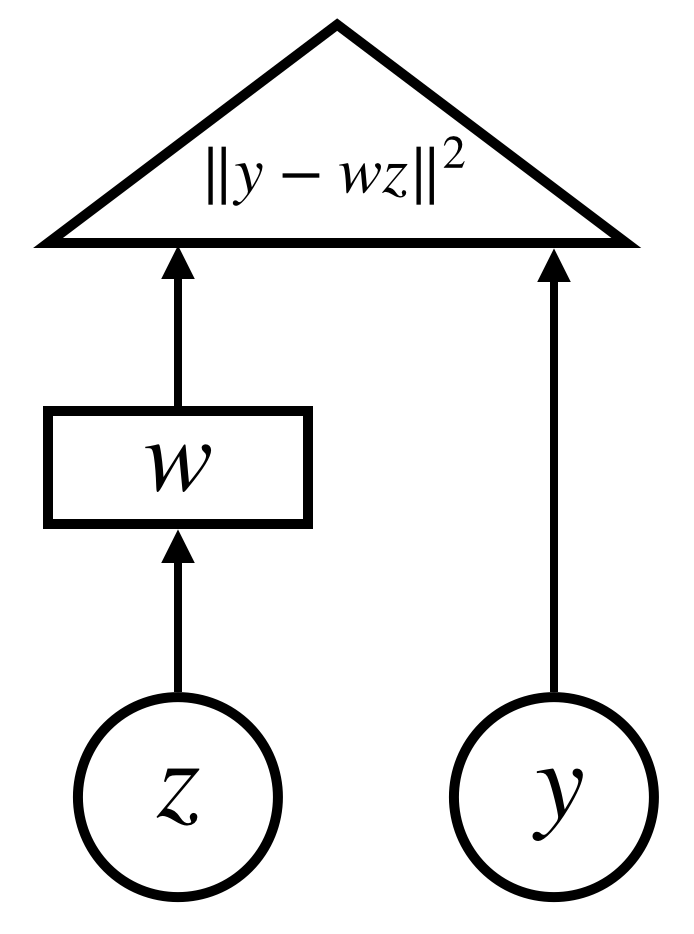
\includegraphics[height=\textwidth]{lectures/10-a/energy-based-1.png}
        \caption{Principal Component Analysis}
        \label{fig:unsupervised-energy-1}
    \end{subfigure}
    \begin{subfigure}[b]{0.4\textwidth}
        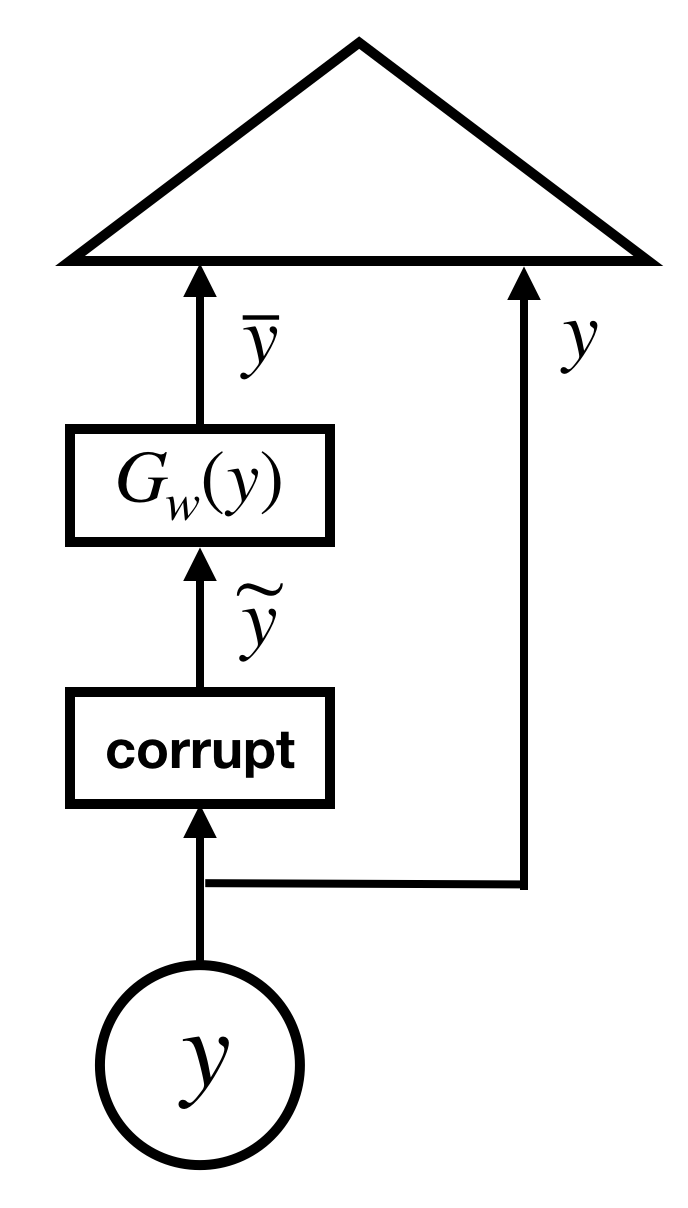
\includegraphics[height=\textwidth]{lectures/10-a/energy-based-2.png}
        \caption{Denoising Autoencoder}
        \label{fig:unsupervised-energy-2}
    \end{subfigure}
    \caption{Shape the Energy Function}\label{fig:unsupervised-energy}
    \end{figure}

    \item \textbf{Push Down and Push Up}: Here are two methods that push down energy of data points while push up elsewhere or on chosen locations, both invented by physicists.
    \begin{enumerate}
        \item \textbf{Monte-Carlo Sampling}: Replace integral with discrete sum, draw samples and take average.
        \item \textbf{Variational Approximation}: Replace $P(y, w)$ distribution with another distribution $Q$ that is easier to compute (e.g. Gaussian), and minimize the Kullback–Leibler divergence between $P$ and $Q$.
    \end{enumerate}

    \item \textbf{Minimize Gradient and Maximize Curvature}: It is impractical. We need to make energy flat around data points, which means the derivative being zero, and the second derivative as large as possible. In other words, "Compute the gradients with respect to parameters of the sum of the diagonal terms which is the trace of the Hessian function with respect to the inputs."

    \item \textbf{Denoising Autoencoder}: This method is useful. How it works is we have an input $y$ and corrupt it with noise, then pass the corrupted $y$ through a parameterized function $G$, eventually the energy function compares the uncorrupted $y$ and $G(\bar{y})$, gives the distance $\bar{y}$ is away from the manifold which is also the reconstruction error. The noise $\bar{y}$ will have high energy. There are two problems with this method, the first one is that it is hard to know what noise to add. There are too many ways to corrupt an input, you may not be able to cover all that expand the entire high-dimensional space outside your manifold. The second one it that there is no guarantee the model is going to learn exactly what you taught, for instance, the catastrophic scenario is that the points reconstructed go in circle. See Figure~\ref{fig:unsupervised-energy-2} above for an illustration.
\end{enumerate}